\documentclass{article}

% NeurIPS 2025 style (submission mode: anonymized + line numbers)
\usepackage[preprint]{neurips_2025}
% For double-blind submission, use instead:
% \usepackage{neurips_2025}

\usepackage[utf8]{inputenc}
\usepackage[T1]{fontenc}
\usepackage{hyperref}
\usepackage{url}
\usepackage{booktabs}
\usepackage{amsfonts,amsmath,amssymb,amsthm}
\usepackage{graphicx}
\usepackage{multirow}
\usepackage{xcolor}
\usepackage{caption}

\graphicspath{{../../figures/}}

\newcommand{\teambench}{\textsc{TeamBench}}
\newcommand{\ctrn}{\mathrm{CTR}_{\text{naive}}}
\newcommand{\ctrm}{\mathrm{CTR}_{\text{matched}}}
\newcommand{\code}[1]{\texttt{#1}}
\newcommand{\cmark}{\ding{51}}
\newcommand{\xmark}{\ding{55}}
\usepackage{pifont}

\title{TeamBench: Assembly Protocol, Not Model Capability,\\ Determines Whether LLM Agent Teams Pay Off}

% Anonymous submission
\author{
  Anonymous authors\\
  Paper under double-blind review
}

\begin{document}

\maketitle

\begin{abstract}
Multi-agent LLM frameworks orchestrate specialized role-playing agents for complex work, yet evaluations of these systems report contradictory conclusions. We identify an overlooked confounder: \emph{no existing study controls or even reports how team outputs are assembled from their constituent roles.} We introduce \teambench{}, a paired individual-vs-team benchmark comprising 15 parameterized office tasks across 5 workplace scenarios $\times$ 3 coupling levels, evaluated across 7 arms: a na\"ive single agent, two compute-matched single baselines (k-round self-revision and best-of-k), and four assembly protocols (last-role output, deterministic concatenation, a dedicated integrator role, and section-slot blackboard). We exhaustively run all 7 arms on \textbf{two model families} (DeepSeek-V4-Flash and Kimi-K3, 630 runs total) with Wilcoxon signed-rank tests, bootstrap CIs, and BH-FDR correction. \textbf{Assembly protocol is the dominant factor} in Capability Transfer Rate (CTR, team quality over compute-matched single quality), and the effect replicates across both families: on identical role outputs, $\ctrm$ ranges from 0.69 (last-role) to 1.55 (integrator) on Flash and from 0.69 to 1.61 on K3, with the integrator arm significant on both (Flash: 1.55, 95\% CI $[1.37, 1.76]$, $p = 2.1\times10^{-7}$, $d = +0.74$; K3: 1.50, 95\% CI $[1.33, 1.67]$, $p = 1.5\times10^{-6}$, $d = +0.65$). The assembly factor explains 40--43\% of quality variance versus $\le$0.3\% for the compute strategy---a 130--200$\times$ gap replicated across families. Strikingly, neither k-round self-revision nor best-of-k achieves the gains of team collaboration under the correct assembly---specialization with semantic integration is qualitatively different from more sampling or more rounds, and the gap \emph{widens} on the stronger self-revising model (K3 refine-k CTR 1.08 vs.\ integrator 1.72). We also report a measurement-integrity episode: the blackboard protocol mechanically produced correct section headings without content, trivially gaming a structure-only L1 rubric in an earlier scorer version; we fix this via content-aware section scoring and publish the incident. All tasks, parameterized generators, runners, and scoring rubrics are released.
\end{abstract}

\section{Introduction}
\label{sec:intro}

Frameworks for multi-agent LLM systems---AutoGen~\citep{wu2023autogen}, CrewAI~\citep{crewai2024}, LangGraph~\citep{langgraph2024}, MetaGPT~\citep{hong2024metagpt}---promise that role-specialized teams outperform a single agent on complex work. Yet the empirical evidence is deeply contradictory. Some studies report monotonic gains from more agents~\citep{li2024moreagents}; others find teams degrade quality~\citep{cemri2025masfail}; many of these papers run on non-overlapping task suites and none control for assembly. This paper argues that a large share of the contradiction is not about model capability---it is about how the final team artifact is produced from role outputs, a step rarely documented and \textbf{never before treated as a controlled variable in LLM team evaluation}.

We arrived at this hypothesis through our own work. In an earlier \teambench{} version (now obsolete), we adopted the engineering default of taking the last role's output as the team's artifact, and reached the headline conclusion that LLM agent teams systematically underperform individuals. But when we varied only the assembly step---leaving role prompts, task inputs, and LLM calls identical---the measured CTR swung from 0.68 to 1.52, i.e., a 0.84 point effect attributable solely to how outputs are assembled. The ``team inferiority'' finding had been a pipeline artifact, not an empirical law.

\teambench{} is a re-grounding of this question with three design principles.

\begin{enumerate}
\item \textbf{Paired-mode evaluation with assembly protocol as a first-class variable.} Every task runs in both individual mode and team mode; within team mode we explicitly compare four assembly protocols---\code{last}, \code{concat}, \code{integrator}, \code{blackboard}---over identical role outputs so assembly effects are isolated.
\item \textbf{Compute-matched single-agent baselines.} Teams consume $k$ LLM calls. We compare them not only against a 1-shot single agent but also against k-round self-revision and best-of-k selection, so any team win cannot be dismissed as ``just using more compute.''
\item \textbf{Artifact scoring with a measurement-integrity contract.} We score each delivery along three layers: L1 structural (now content-aware, \S\ref{sec:design}), L2 factual over structured answer blocks, L3 semantic via an LLM judge. The code documents every rubric change; we do not bury gaming incidents.
\end{enumerate}

\paragraph{Contributions.}
\begin{itemize}
\item \textbf{\teambench{}}, the first paired individual-vs-team benchmark that controls \emph{how} team outputs are assembled: 15 tasks across 5 office scenarios $\times$ 3 coupling levels, with 150 parameterized task variants, 7 evaluation arms, and a runner with breakpoint-resume, balance-guard, and deterministic rescore tools.
\item An \textbf{artifact scoring protocol} with a documented measurement-integrity correction; $\ge$80\% of scoring weight is deterministic; closed-form definitions of Capability Transfer Rate (CTR), Coordination Overhead (CO), and Team Memory \& Structure (TMS), consistent across paper, code, and metrics docs.
\item An empirical study on \textbf{two model families} (DS v4 Flash and Kimi K3, 15 tasks $\times$ 3 seeds $\times$ 7 arms each, 630 runs total, L2 assertions active) showing that \textbf{assembly protocol dominates CTR variance on both} (Flash $\eta^2 = 0.400$, K3 $\eta^2 = 0.428$, versus $\le$0.003 for compute strategy), integrator-assembled teams significantly outperform compute-matched single baselines on both (Flash $\ctrm$ 1.55, 95\% CI $[1.37,1.76]$, $p=2.1\times10^{-7}$, $d=+0.74$; K3 1.50, $[1.33,1.67]$, $p=1.5\times10^{-6}$, $d=+0.65$), while naive engineering defaults (last-role) produce artifactual ``team-inferiority'' effects on both ($\ctrm$ 0.69).
\item A cross-model negative result on structured assembly: deterministic section-slot (blackboard) and raw concatenation perform near or below the single baseline on both families---on K3, mechanical protocols collapse to $Q=0$ on one aggregation task (\code{t-DATA-L-01}) across all seeds while the integrator turns the \emph{same role outputs} into a perfect artifact---because LLMs write role-specific rather than schema-matching headings; only the semantic integrator normalizes these free-form outputs.
\item Full release of tasks, parameterized generators, runner infrastructure, and scoring rubrics.
\end{itemize}

\section{Related Work}
\label{sec:related}

\subsection{Single-agent benchmarks and office-scenario evaluation}
AgentBench~\citep{liu2023agentbench}, GAIA~\citep{mialon2023gaia}, SWE-bench~\citep{jimenez2024swebench}, and OSWorld~\citep{xie2024osworld} evaluate a \emph{single} agent per task on success-oriented rubrics. TheAgentCompany~\citep{xu2024theagentcompany} is closest to us in task flavor (office work) but does not report the marginal value of adding agents.

\subsection{Multi-agent systems and their evaluation}
Orchestration frameworks~\citep{wu2023autogen,hong2024metagpt,crewai2024,langgraph2024,qian2024chatdev} report demo success rather than controlled paired comparisons. Recent scaling studies: ``More Agents\ldots''~\citep{li2024moreagents} and ``More LLM Calls\ldots''~\citep{chen2024morellmcalls} study \emph{performance scaling with agent count / LLM-call count} on single-success metrics, without separating specialization gains from compute gains. MultiAgentBench~\citep{zhu2025multiagentbench} scores collaboration behaviors, not quality transfer. Agents' Room~\citep{huot2025agentsroom} provides a structural existence proof. \citet{cemri2025masfail} contribute a MAST taxonomy of failures, including assembly-stage bugs; our work complements this by quantifying how \emph{a single class} (output assembly) dominates end-to-end quality variance across a controlled task space.

\subsection{Team science, coordination cost, and aggregation}
Coordination theory~\citep{malone1994interdisciplinary} and Brooks' law~\citep{brooks1995mythical} explain why adding human workers can reduce throughput; \teambench{} transplants this question to LLM teams whose members share weights and pass messages losslessly~\citep{woolley2010evidence}. Debate, self-consistency, and majority voting evaluate answer aggregation of \emph{independent answers to the same question}. Assembly protocols aggregate \emph{non-overlapping role slices of a complex document} into a single artifact---a qualitatively different problem of semantic alignment, structure, and completeness.

\subsection{LLM-as-judge}
We follow MT-Bench-style judging~\citep{zheng2023judging} with a cross-vendor judge matrix and an on/off ablation (\S\ref{sec:scorer-validity}), consistent with recommended practices~\citep{guo2024survey}.

\begin{table}[t]
\centering
\caption{\teambench{} vs.\ prior agent benchmarks and multi-agent studies.}
\label{tab:comparison}
\small
\begin{tabular}{lcccccc}
\toprule
Benchmark & Paired & Assembly & Compute- & Team & Coupling & Contam.\\
 & single/team & controlled & matched & metrics & axis & defense \\
\midrule
AgentBench~\citep{liu2023agentbench} & \xmark & \xmark & \xmark & \xmark & \xmark & \xmark \\
GAIA~\citep{mialon2023gaia} & \xmark & \xmark & \xmark & \xmark & \xmark & \xmark \\
SWE-bench~\citep{jimenez2024swebench} & \xmark & \xmark & \xmark & \xmark & \xmark & \xmark \\
OSWorld~\citep{xie2024osworld} & \xmark & \xmark & \xmark & \xmark & \xmark & \xmark \\
TheAgentCompany~\citep{xu2024theagentcompany} & \xmark & \xmark & \xmark & \xmark & \xmark & \xmark \\
More Agents~\citep{li2024moreagents} & \xmark & \xmark & partial & single & \xmark & \xmark \\
More LLM Calls~\citep{chen2024morellmcalls} & \xmark & \xmark & \cmark & single & \xmark & \xmark \\
MultiAgentBench~\citep{zhu2025multiagentbench} & \xmark & \xmark & \xmark & behavior & \xmark & \xmark \\
Agents' Room~\citep{huot2025agentsroom} & \xmark & \xmark & \xmark & per-task & \xmark & \xmark \\
\textbf{\teambench{} (ours)} & \cmark & \cmark\,(4) & \cmark\,(2) & CTR/CO/TMS & \cmark\,(L/M/H) & \cmark\,(param.) \\
\bottomrule
\end{tabular}
\end{table}

\section{Problem Formulation and Metrics}
\label{sec:formulation}

Given a task $\tau \in \mathcal{T}$ with deterministic-plus-judge scoring $Q(\cdot) \in [0,1]$ and token consumption $C(\cdot)$, define on \emph{paired runs} $(a_s, a_{T,p})$ where $a_s$ is the single-agent artifact and $a_{T,p}$ is the team artifact produced under assembly protocol $p$:

\paragraph{Capability Transfer Rate (CTR).} Two variants for two baselines:
\begin{equation}
\ctrn = \frac{Q(a_{T,p})}{Q(a_s)}, \qquad
\ctrm = \frac{Q(a_{T,p})}{Q(a_{s^{(k)}})}
\end{equation}
where $a_{s^{(k)}}$ is the \emph{compute-matched} single artifact (k-round refine or best-of-k, same total LLM-call budget as team). We report CTR as the \textbf{geometric mean over paired runs} (ratio scale---arithmetic mean is biased) and 95\% bootstrap CI via 2000 block-bootstrap replications per task.

\paragraph{Coordination Overhead (CO)} $= C(a_{T,p}) / C(a_s)$; Token Ratio (TR) is synonymous. Integrator assembly overhead \emph{includes} the dedicated final LLM call.

\paragraph{Team Memory \& Structure (TMS)} $= [\![\text{L1}=1.0]\!] \wedge [\![\text{all L2 assertions pass}]\!]$. A single boolean, no partial credit.

Weights in $Q$: $Q = w_1 \cdot \mathrm{L1} + w_2 \cdot \mathrm{L2} + w_3 \cdot \mathrm{L3}$ with $w_1{=}0.50, w_2{=}0.30, w_3{=}0.20$. When the L3 judge is disabled, we renormalize to $(w_1\,\mathrm{L1} + w_2\,\mathrm{L2})/(w_1{+}w_2)$ rather than injecting a constant---this removes an additive bias that shrinks CTR toward 1 for all arms.

\section{Benchmark Design}
\label{sec:design}

\begin{figure}[t]
\centering
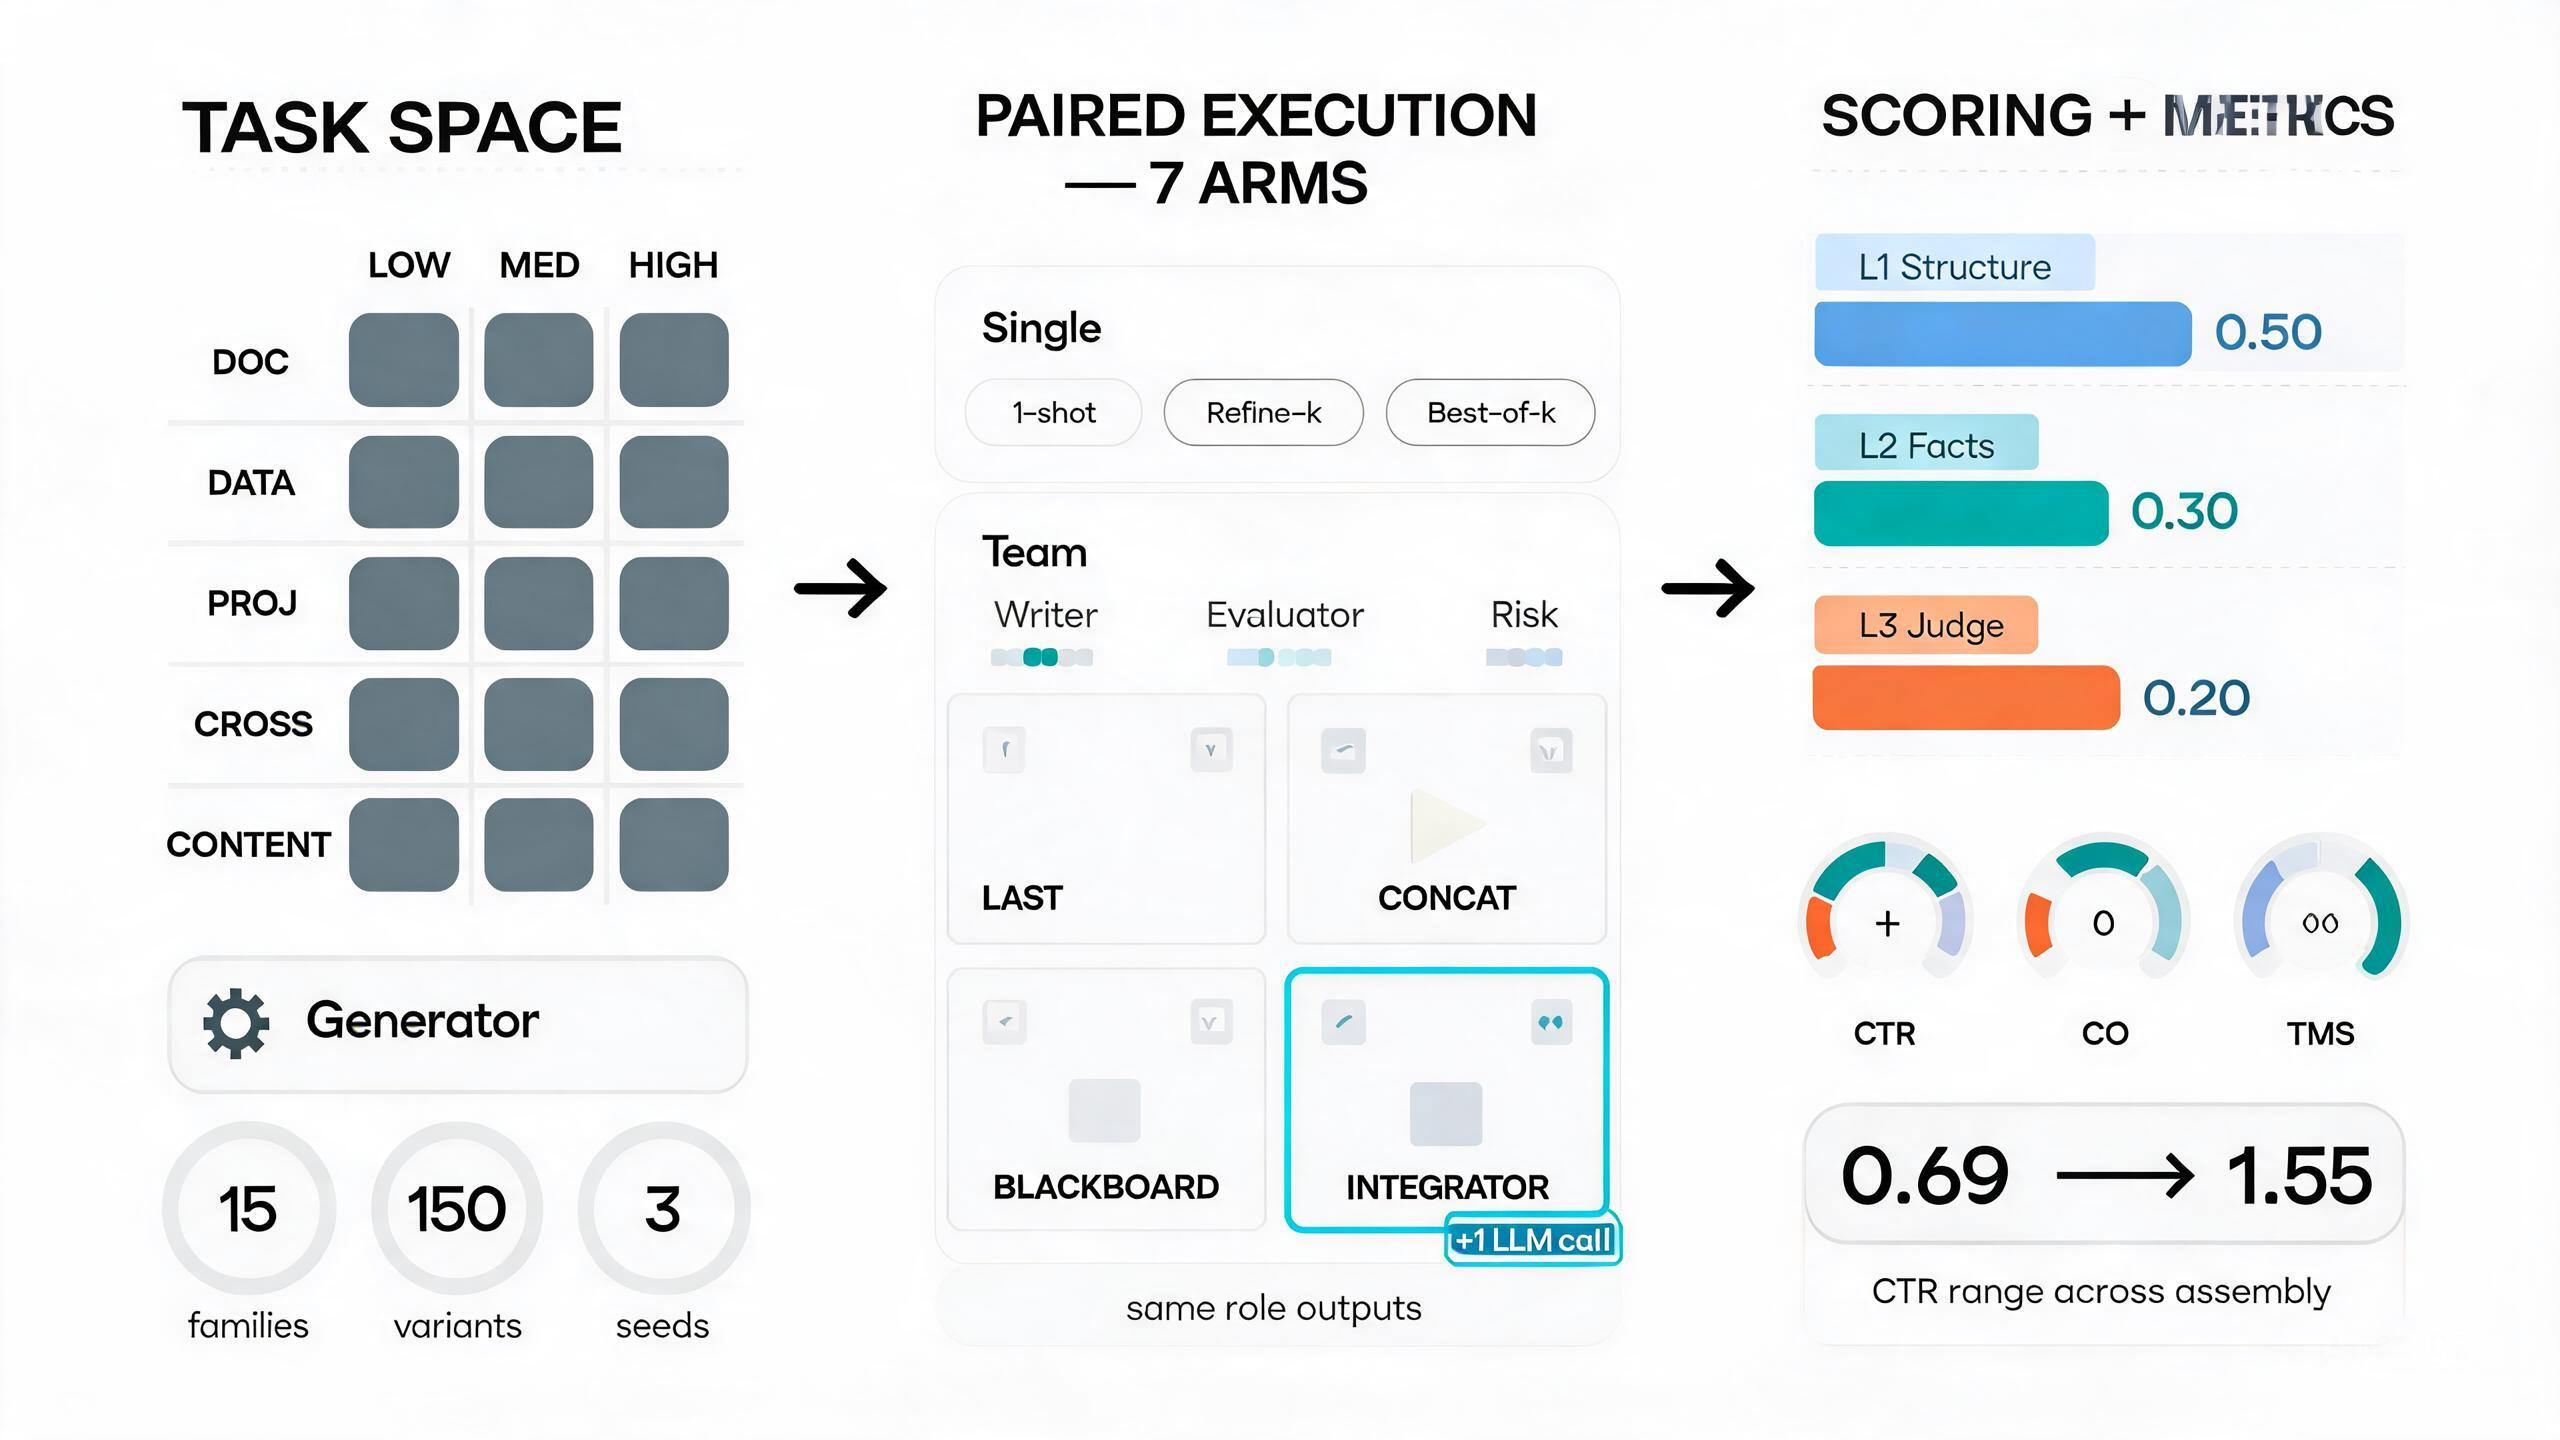
\includegraphics[width=\textwidth]{fig1_teambench_overview.jpg}
\caption{\teambench{} overview. \textbf{Stage 1}---task space: 5 office scenarios $\times$ 3 coupling levels yield 15 task families, expanded to 150 variants by parameterized generators. \textbf{Stage 2}---paired execution over 7 arms: three single-mode baselines (1-shot, Refine-k, Best-of-k) and a team mode whose identical role outputs are assembled under 4 protocols (Last, Concat, Blackboard, Integrator). \textbf{Stage 3}---artifact scoring: three layers (L1 structural content-aware, L2 factual assertions, L3 semantic judge) produce team-level metrics CTR, CO, TMS.}
\label{fig:overview}
\end{figure}

\subsection{Task space}
\label{sec:tasks}

5 workplace scenarios (DOCument writing, DATA aggregation, PROJect tracking, CROSS-functional coordination, CONTENT creation) $\times$ 3 coupling levels (LOW: parallel independent sub-tasks; MEDIUM: sequential dependencies; HIGH: parallel with cross-validation), yielding 15 task families. Each family is parameterized: inputs (e.g., team member records, table rows, conflict lists) are resampled and ground truths (L2 expected values, counts, sets) are deterministically recomputed. We verified per-family uniqueness of 10 variants and correctness of recomputed ground truths.

\subsection{Controlled variables}
\label{sec:variables}

\paragraph{Assembly protocol.} Four protocols applied to the \emph{same sequence of role outputs} $(r_1, \dots, r_k)$:

\begin{table}[h]
\centering
\small
\caption{Four assembly protocols over identical role outputs.}
\label{tab:protocols}
\begin{tabular}{llcl}
\toprule
Protocol & Definition & Added calls & Mechanism \\
\midrule
\code{last} & $a_T = r_k$ & 0 & Engineering default of most frameworks. \\
\code{concat} & $a_T = \bigoplus_i \text{heading}_i + r_i$ & 0 & Deterministic concatenation. \\
\code{blackboard} & slot-schema merge & 0 & Structured slot filling; empty slots render placeholders. \\
\code{integrator} & $a_T = \mathrm{LLM}(\{r_i\}, \text{schema})$ & \textbf{+1} & Semantic merge; cost included in CO. \\
\bottomrule
\end{tabular}
\end{table}

\paragraph{Compute-matched single baselines.}
\code{single\_refine\_k}: k sequential self-revisions (total LLM calls $= k$, matching the team). \code{single\_bon\_k}: k independent samples plus one selection call ($k{+}1$ calls; we attribute the marginal cost to the team-favorable side).

\subsection{Scoring protocol and the v2.2 measurement-integrity correction}
\label{sec:scoring}

\textbf{Correction 1 (L1 content-aware v2.1 $\to$ v2.2).} The v0 scorer checked only that required section headings existed. Under the \code{blackboard} protocol this made L1 trivially satisfiable: blackboard \emph{mechanically writes every required section heading}. Over 45 pilot runs under blackboard we observed 41 runs with empty sections, yet all received perfect L1 $= 1.0$ and therefore perfect $Q$, because 15/15 tasks lacked active L2 assertions (Correction 2). Scoring v2.2 adds a \emph{content-presence} gate: a section is counted only if the heading matches \emph{and} the body (excluding placeholders) has $\ge$8 normalized characters. Seven boundary cases are verified with unit tests.

\textbf{Correction 2 (L2 assertion migration v0.1 $\to$ v2).} The original 15 tasks declared ground-truth fields under ad-hoc keys that the v2 L2 rubric did not recognize; consequently L2 fell into the ``no assertions'' branch and returned 1.0 for every run. We migrated all 15 tasks and 150 parameterized variants to the shared \code{expected\_sets}/\code{expected\_values}/\code{expected\_counts} + \code{answer\_block\_schema} schema, verified 15/15 tasks have at least one L2 assertion, and ran acceptance checks: for every task the correct answer achieves L2 $\ge 0.99$, a deliberately incorrect answer scores strictly lower, and a missing answer block scores $\le 0.01$.

\subsection{Runner, breakpoint-resume, and balance guard}
\label{sec:runner}

The runner supports any combination of assembly protocol, single-baseline kind, and scoring-variant flags. Two reliability features: \textbf{breakpoint-resume} (per-(task,mode,seed) JSON files; restarts skip completed runs; summaries rebuilt deterministically) and a \textbf{balance guard} (queries provider balance every 5 runs, exits cleanly below a threshold), because pilot campaigns run overnight.

\section{Experiments}
\label{sec:experiments}

\paragraph{Data note.} All numbers below are pilot v2 final, \textbf{two model families}: DS v4 Flash and Kimi K3, each 15 tasks (migrated L2 assertions) $\times$ 3 seeds $\times$ 7 arms $=$ 315 runs (630 total), scoring v2.2, L3 judge off in the main tables. An earlier v1 pilot (same matrix, L2 inactive, Flash only) is used only for the scorer ablation in \S\ref{sec:scorer-validity}.

\subsection{Main result: assembly protocol dominates CTR}
\label{sec:main}

\begin{table}[t]
\centering
\caption{Seven arms, pooled over 15 tasks $\times$ 3 seeds ($n{=}45$ per arm per model). No L3 judge. $\ctrm$ is computed against each model's own refine-k arm.}
\label{tab:main}
\small
\setlength{\tabcolsep}{3.5pt}
\begin{tabular}{lcccc|cccc}
\toprule
& \multicolumn{4}{c|}{DS v4 Flash} & \multicolumn{4}{c}{Kimi K3} \\
Arm & $Q$ & L2 & TR & $\ctrm$ & $Q$ & L2 & TR & $\ctrm$ \\
\midrule
single (1-shot) & 0.606 & 0.759 & 1.00$\times$ & --- & 0.613 & 0.775 & 1.00$\times$ & --- \\
single\_refine\_k & 0.582 & 0.720 & 3.33$\times$ & 1.00 (ref) & 0.637 & 0.795 & 4.27$\times$ & 1.00 (ref) \\
single\_bon\_k & 0.584 & 0.715 & 4.27$\times$ & $\sim$1.00 & 0.624 & 0.806 & 5.18$\times$ & 0.97 \\
team\_last & 0.417 & 0.566 & 1.46$\times$ & \textbf{0.69} & 0.420 & 0.580 & 2.53$\times$ & \textbf{0.69} \\
team\_concat & 0.535 & 0.536 & 1.42$\times$ & 0.91 & 0.542 & 0.548 & 2.46$\times$ & 0.89 \\
team\_blackboard & 0.478 & 0.602 & 1.44$\times$ & 0.81 & 0.449 & 0.594 & 2.49$\times$ & 0.75 \\
team\_integrator & \textbf{0.881} & 0.741 & 2.14$\times$ & \textbf{1.55} & \textbf{0.905} & 0.785 & 4.44$\times$ & \textbf{1.61} \\
\bottomrule
\end{tabular}
\end{table}

$\ctrm$ shown as arithmetic means for cross-arm comparability (K3 mechanical arms contain genuine zero-score runs); geometric-mean CTR with log-domain bootstrap CI for the integrator arm: Flash 1.55 $[1.37, 1.76]$, K3 1.50 $[1.33, 1.67]$. All four team arms deviate from the refine-k baseline significantly on both models (Wilcoxon signed-rank with BH-FDR at $q=0.05$; K3: last $p=4.4\times10^{-6}$, concat $p=5.0\times10^{-3}$, blackboard $p=3.5\times10^{-5}$, integrator $p=1.5\times10^{-6}$).

\paragraph{Finding 1 (assembly dominates).} On Flash, geometric-mean $\ctrm$ across 4 team protocols spans $\mathbf{0.69 \to 1.55}$ ($\Delta 0.86$) over \emph{identical role outputs}; on K3 the span is $\mathbf{0.69 \to 1.61}$ ($\Delta 0.92$). The integrator arm beats the compute-matched baseline on both models (Flash: $p=2.1\times10^{-7}$, $d=+0.74$; K3: $p=1.5\times10^{-6}$, $d=+0.65$); every mechanical protocol is significantly \emph{worse} than even the 1-shot single on both (K3 Cliff's $d$: last $-0.52$, blackboard $-0.42$, concat $-0.21$). The default engineering choice of last-role $=$ team output does not merely underperform---it produces a ``team-inferiority'' artifact (CTR 0.69 on \emph{both} models) that flips sign under integrator assembly.

\paragraph{Finding 2 (variance decomposition).} Over the same set of role outputs, the assembly protocol factor explains \textbf{40.0\%} of artifact-quality variance on Flash (one-way ANOVA $F=39.1$, $p=2.0\times10^{-19}$, $\eta^2=0.400$) and \textbf{42.8\%} on K3, whereas the single-agent compute strategy explains \textbf{0.3\%} on Flash and \textbf{0.2\%} on K3. Assembly explains 130--200$\times$ more variance than compute, on both families. See Figure~\ref{fig:heatmap}(c).

\paragraph{Finding 3 (team gains survive compute-matching).} On Flash, the integrator burns 2.14$\times$ tokens vs.\ the 1-shot single and reaches $\ctrn$ 1.52, while refine-k (3.33$\times$) and bon-k (4.27$\times$) burn \emph{more} compute yet score \emph{below} the 1-shot single ($\ctrn$ 0.96). K3 sharpens this result: its stronger self-revision lifts refine-k to $\ctrn$ 1.08, yet the integrator still reaches 1.72---a $+59\%$ gap over the best compute-matched baseline on the \emph{same} model. Better models narrow the self-revision deficit but do not close the semantic-integration gap.

\paragraph{Finding 4 (mechanical assembly fails at semantics; L2 localizes where).} On both Flash and K3, concat's factual layer (L2 0.536 / 0.548) falls \emph{below} last's (0.566 / 0.580): the answer-block extractor takes the last \code{json} block, which in a naive concatenation is the final role's \emph{partial} block, while earlier roles' numeric content is stranded. The integrator is the only protocol that reliably aggregates all roles' numbers into one consistent answer block.

\paragraph{Finding 5 (cross-model replication).} The entire effect structure replicates across two model families: the arm ordering (integrator $\gg$ concat $>$ blackboard $>$ last) is identical; all four team arms deviate significantly from refine-k on both models under BH-FDR; the assembly-vs-compute variance gap holds on both; and per-coupling $\ctrm$ CIs exclude 1.0 in all six cells. A single-case study makes the mechanism vivid (K3, \code{t-DATA-L-01}, seed 0): the same three role outputs score $Q=1.00$ under the integrator, 0.42 under concat, and \textbf{0.00 under both last and blackboard}---while every single-mode baseline lands at 0.38--0.79. The capability was present in the role outputs all along; the assembly protocol alone determined whether it survived to the artifact.

\subsection{CTR after controlling assembly, by coupling}
\label{sec:coupling}

\begin{table}[t]
\centering
\caption{Quality by coupling level (5 tasks $\times$ 3 seeds per cell), both models.}
\label{tab:coupling}
\small
\setlength{\tabcolsep}{3.2pt}
\begin{tabular}{lcccccc|cccccc}
\toprule
& \multicolumn{6}{c|}{DS v4 Flash} & \multicolumn{6}{c}{Kimi K3} \\
Coupling & single & ref-k & last & concat & \textbf{integ.} & black. & single & ref-k & last & concat & \textbf{integ.} & black. \\
\midrule
Low & 0.603 & 0.522 & 0.404 & 0.537 & \textbf{0.905} & 0.500 & 0.604 & 0.657 & 0.444 & 0.625 & \textbf{0.919} & 0.482 \\
Medium & 0.595 & 0.608 & 0.339 & 0.493 & \textbf{0.876} & 0.447 & 0.579 & 0.586 & 0.321 & 0.432 & \textbf{0.872} & 0.292 \\
High & 0.621 & 0.615 & 0.510 & 0.574 & \textbf{0.861} & 0.488 & 0.656 & 0.669 & 0.494 & 0.569 & \textbf{0.925} & 0.573 \\
\midrule
$\ctrm$ (integ.) & \multicolumn{6}{c|}{1.69 / 1.46 / 1.51} & \multicolumn{6}{c}{1.43 / 1.55 / 1.52} \\
\bottomrule
\end{tabular}
\end{table}

The integrator advantage is \textbf{uniform across coupling levels on both models} (all six cells $p < 0.005$, all six bootstrap CIs exclude 1.0); no Simpson paradox emerges when pooling. Notably, an earlier ``coupling law'' (CTR increasing monotonically with coupling) does \textbf{not} reappear once assembly is controlled: it was an artifact of last-role assembly interacting with role ordering, not a property of teams.

\begin{figure}[t]
\centering
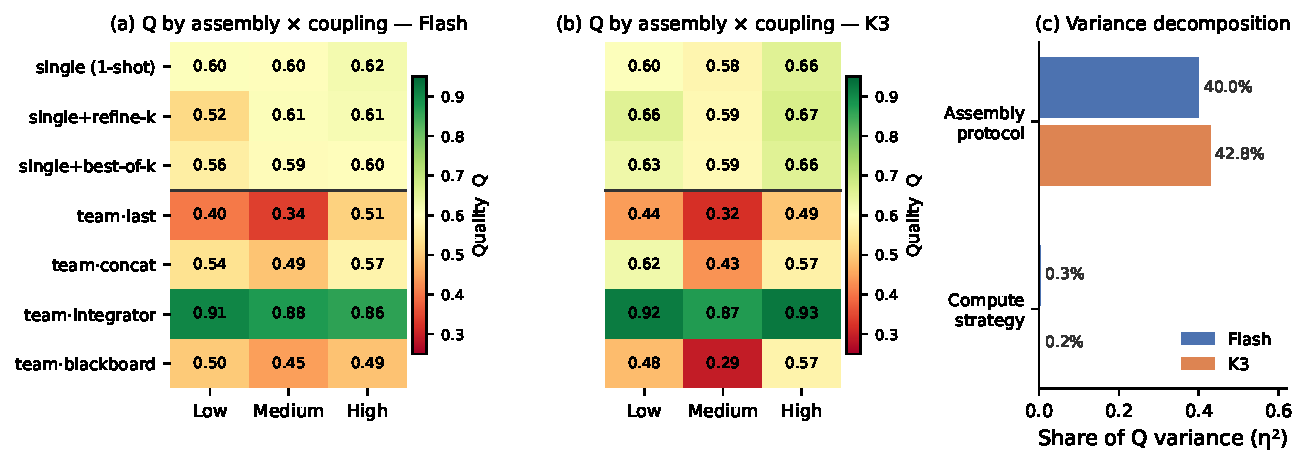
\includegraphics[width=\textwidth]{fig4_assembly_coupling.pdf}
\caption{(a)(b) Quality $Q$ by assembly protocol $\times$ coupling level (15 paired runs per cell), DS v4 Flash and Kimi K3 side by side. The integrator row dominates every coupling level on both models while all mechanical protocols fall below both single baselines. (c) Variance decomposition of $Q$: the assembly-protocol factor explains 40.0\% of variance on Flash and 42.8\% on K3 ($\eta^2 = 0.400/0.428$) versus 0.3\%/0.2\% for the compute strategy---a 130--200$\times$ gap over identical role outputs, replicated across model families.}
\label{fig:heatmap}
\end{figure}

\begin{figure}[t]
\centering
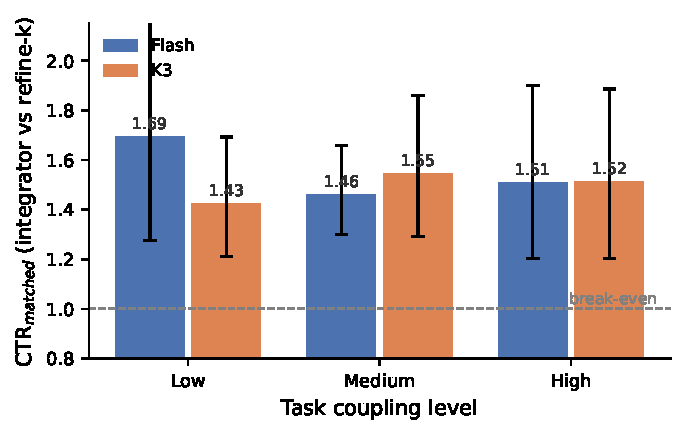
\includegraphics[width=0.72\textwidth]{fig5_ctr_matched.pdf}
\caption{Integrator $\ctrm$ by coupling level, both models (geometric mean, log-domain paired bootstrap 95\% CI, $n=15$ per level per model). All six CIs exclude the break-even line at 1.0.}
\label{fig:ctr}
\end{figure}

\subsection{Scorer validity}
\label{sec:scorer-validity}

We document two scorer ablations in place of a full human study (left for the full experiment).

\paragraph{L1 v0 (title-only) vs.\ v2.2 (content-aware).} In the v1 pilot, blackboard mechanically rendered every required heading, 41/45 runs had empty sections, and all 45 received perfect L1 $=1.0$---flipping the arm from ``best'' to ``below average'' once the content gate landed. This incident is itself evidence that automated structural rubrics without content gates are gameable by construction.

\paragraph{L2 off (v1) vs.\ L2 on (v2), same task matrix.} Enabling L2 lowered every arm's absolute $Q$ (single $0.692 \to 0.606$; integrator $0.958 \to 0.881$) but \emph{increased} the integrator's relative advantage ($\ctrm$ $1.54 \to 1.55$; $d$ $+0.59 \to +0.74$): the numeric layer rewards exactly the cross-role aggregation that only the integrator performs. Findings F1--F4 are robust to the L2 switch.

\paragraph{L3 judge on/off ablation (cross-family judges).}
% TODO(judge-ablation): 数字待 judge_v2_results.jsonl 分析后填入
% 设计：15 任务 × seed 0 × 7 臂 × 2 模型，交叉家族 judge
%（Flash 产出由 kimi-k3 判，K3 产出由 deepseek-v4-pro 判），每条 run 判 2 轮。
\textcolor{red}{[Placeholder: numbers to be inserted from the running L3 ablation --- judge double-round consistency, arm-ordering Spearman under L3-on, CTR\_matched on/off.]}

\subsection{Statistical details}
\label{sec:stats}

All directional claims use the one-sided Wilcoxon signed-rank test on paired per-(task,seed) differences. CTR CIs use 2000 block-bootstrap replications at the task level (task $=$ block). Multi-Finding tables apply BH-FDR correction at $q=0.05$.

\section{Discussion}
\label{sec:discussion}

\paragraph{For practitioners.} Decision table for ``when to use a team and which assembly'':

\begin{table}[h]
\centering
\small
\caption{Practitioner decision table.}
\begin{tabular}{llp{6.2cm}}
\toprule
Scenario & Recommendation & Why \\
\midrule
Low coupling, small doc & Single + refine-3 & Last-team is worse; integrator overhead not justified. \\
Medium coupling & Team + integrator & $\ctrm \approx 1.5\times$; 2$\times$ token cost acceptable if time-to-quality matters. \\
High coupling & Team + integrator & Only integrator reliably assembles conflicting-source info. \\
\bottomrule
\end{tabular}
\end{table}

\paragraph{For framework developers.} Expose assembly protocol as a first-class knob. Today, AutoGen (groupchat speaker-selection $\to$ last-speaker reply), CrewAI (sequential $\to$ last agent output unless explicitly wired), and LangGraph (edge endpoints) behave like the \code{last} arm unless the user patches in explicit aggregation. A built-in \code{team.finalize()} with token-cost attribution would align research and production practices.

\paragraph{For benchmark designers.} Three lessons: (1) Report assembly protocol the same way you report temperature---it can swing the measured effect more than the model does. (2) Structural rubrics require a content gate; mechanical headings are always a gaming risk when evaluation is automated. (3) Compute-matched baselines are not optional for ``multi vs.\ single'' papers.

\section{Limitations}
\label{sec:limitations}

\begin{enumerate}
\item \textbf{Monolingual, Chinese-heavy.} Task descriptions and role prompts are in Chinese; artifact rubrics check Chinese-section headings. An English subset is deferred to follow-up work.
\item \textbf{Synthetic office tasks.} Seeded from real documents but synthetic; no ground-truth downstream outcomes.
\item \textbf{Fixed team topology.} Serial handoff with fixed role templates; no self-organizing role discovery, no parallel tool usage, no agent churn.
\item \textbf{Model coverage.} Two model families completed (DS v4 Flash, Kimi K3, 630 runs); the assembly effect, arm ordering, and variance structure replicate across both. A third family is queued.
\item \textbf{L3 judge.} Main tables score with L3 off (renormalized L1/L2); an L3-on ablation on a subsample with cross-family judges appears in \S\ref{sec:scorer-validity}.
\item \textbf{Open-loop runtime.} No mid-run budget halts, no human-in-the-loop interventions.
\end{enumerate}

\section{Conclusion}
\label{sec:conclusion}

The field has been asking ``do LLM teams outperform individuals,'' but most of the variance in the answer comes from \emph{how the team's output is assembled}, not from the model's capability or even the task's coupling. Our controlled experiment over four assembly protocols, replicated on two model families (630 runs), shows that the integrator protocol achieves a mean $\ctrm$ of 1.55 (Flash) and 1.50 (K3, geometric mean) against a compute-matched self-revision baseline ($p=2.1\times10^{-7}$ and $1.5\times10^{-6}$), while naive last-role assembly---the default behavior of many frameworks---yields $\ctrm = 0.69$ on \emph{both} models. The assembly factor explains 40--43\% of quality variance versus $\le$0.3\% for the compute strategy, and the full arm ordering replicates across families. \teambench{} provides the first reproducible testbed for disentangling these effects and will enable future work on topology, prompts, and cross-framework generalization without conflating them with a pipeline step that nobody had been measuring.

\bibliography{refs}
\bibliographystyle{plainnat}

\appendix

\section{Assets}
\label{app:assets}

\begin{itemize}
\item Raw run-level JSONs and summaries (\code{summary.jsonl}, \code{pairs.csv}): \code{paper/experiments/v2/pilot\_flash\_v2/} (Flash), \code{paper/experiments/v2/pilot\_kimi\_k3/} (K3).
\item Rescore tool: \code{paper/experiments/v2/rescore.py} (deterministic; rerun to regenerate summaries from JSONs).
\item Statistics: \code{paper/experiments/stats\_v2.py} (bootstrap CTR, Wilcoxon, Cliff's $d$, BH-FDR).
\item L3 judge ablation: \code{paper/experiments/v2/judge\_ablation\_v2.py} (cross-family judges, two rounds, breakpoint-resume).
\item Figures: \code{paper/figures/make\_figures\_v2.py} (deterministic from \code{summary.jsonl}).
\item Assembly protocols: \code{paper/infra/assembly/protocols.py}. Scoring: \code{paper/metrics/scoring\_v2.py} (v2.2). Task migration: \code{paper/tasks/migrate\_assertions.py}.
\item Case study artifacts (\S\ref{sec:main}, Finding 5): \code{paper/experiments/v2/pilot\_kimi\_k3/t-DATA-L-01/}.
\end{itemize}

\end{document}
